\documentclass[french, 12pt]{article}%


\usepackage[T1]{fontenc}
\usepackage[utf8]{inputenc}
\usepackage[french]{babel}

\usepackage{textcomp}

\usepackage[official]{eurosym}

\usepackage{appendix}
\usepackage{pdfpages}

%%%%%%%%%%%%%%%%%%%%%%%%%%%%%%%%%%%%%%%%%%%%%%%%%%%%%%%%%
\newcommand{\itemE}{\item[$\bullet$]}

\newcommand{\titreSeq}{SNMP}
\newcommand{\lycee}{Lycée Brocéliande}
\newcommand{\classSeq}{CIEL }
\newcommand{\matiereSeq}{IR}      
\newcommand{\numSeq}{Cyber}
\newcommand{\numAct}{01}
\newcommand{\objSeance}{Comprendre le principe de SNMP et le mettre en place avec Prometheus}

\newcommand{\moySeq}{\begin{itemize}	
\itemE Machine Kali
\itemE VM entreprise (Metasploitable)
\end{itemize}}

\newcommand{\compSeq}{\begin{itemize}
\item  
\end{itemize}}
%%%%%%%%%%%%%%%%%%%%%%%%%%%%%%%%%%%%%%%%%%%%%%%%%%%%%%%%%%

%%%%%%%%%%%%%%%%%%%%%%%%%%%%%%%%%%%%%%%%%%%%%%%%%%%%%%%%
%%%%Algo
\usepackage[linesnumbered, french]{algorithm2e}
\SetKwFor{For}{Pour}{faire}{fin}
\SetKwFor{While}{Tant que}{faire}{fin}%
\SetKw{KwTo}{à}
\SetKw{KwPas}{par pas de}
\SetKw{KwRet}{Retourne}
\SetKwProg{Fn}{Fonction }{ arguments }{fin}
\SetKwRepeat{Repeat}{Répéter}{jusqu'à}%
\SetKwIF{If}{ElseIf}{Else}{Si}{alors}{Sinon si}{Sinon}{Fin}


\usepackage{listings} %%%%Présenration code source
\lstset{language=C++,
    %numbers=left,
   %stepnumber=1,
    showstringspaces=false,
    tabsize=1,
    breaklines=true,
    breakatwhitespace=false,
    basicstyle=\footnotesize,
    keywordstyle=\color{blue}\footnotesize,
    stringstyle=\color{red}\footnotesize,
    commentstyle=\color{magenta}\footnotesize,
    morecomment=[l][\color{magenta}]{\#}
    }
\lstdefinestyle{commande}{
  basicstyle=\ttfamily\footnotesize,
  keywordstyle=\color{blue},
  commentstyle=\color{gray},
  %numbers=left,
  %numberstyle=\tiny\color{gray},
  numbersep=5pt,
  breaklines=true,
  frame=single,
  backgroundcolor=\color{lightgray!10}
  %captionpos=b,
  %caption=\lstname  
}
%\usepackage[T1]{fontenc}


%\usepackage[T1]{fontenc}

\newcommand{\itemB}{\item[$\Box$]}
% Margins
\topmargin=-0.45in
\evensidemargin=0in
\oddsidemargin=0in
\textwidth=6.5in
\textheight=9.0in
\headsep=0.25in 


\linespread{1.1} 
\usepackage{amsmath}%
\usepackage{amsfonts}%
\usepackage{amssymb}%
\usepackage{graphicx}
\usepackage{lastpage}
\usepackage{enumitem}

%\usepackage[T1]{fontenc}    
\usepackage{multirow}
\usepackage{lscape}
\usepackage[colorlinks = true,
            linkcolor = blue,
            urlcolor  = blue,
            citecolor = blue,
            anchorcolor = blue]{hyperref}
\usepackage{array}
\usepackage{mwe}
%-------------------------------------------
\newtheorem{theorem}{Theorem}
\newtheorem{summary}[theorem]{Summary}
\newenvironment{proof}[1][Proof]{\textbf{#1.} }{\ \rule{0.5em}{0.5em}}



\usepackage{xcolor}

\usepackage{colortbl}
\definecolor{vert_capet}{RGB}{191,255,191}	
\definecolor{bleu_snir}{RGB}{101,191,179}	
\setlength{\doublerulesep}{\arrayrulewidth}
%-------------------------------------------
%%%%%%%%%%%%%%%%%%%%%%%%%%%%%%%%%%%%%%%%%%%%%
\usepackage[framemethod=tikz]{mdframed}
\usepackage{tikz, xcolor, lipsum}
\makeatletter
\mdfsetup{skipabove=\topskip,skipbelow=\topskip}

\tikzset{titre_bleu_snir/.style =
	{draw=bleu_snir, line width=1.5pt, fill=white,
	rectangle, rounded corners, right,minimum height=2em}}
\newcommand{\titreencadre}{Titre}
\makeatletter
\mdfdefinestyle{encadrestyle}{%
	linewidth=1.5pt,roundcorner=5pt,linecolor=bleu_snir,
	apptotikzsetting={\tikzset{mdfbackground/.append style ={%
		fill=white}}},
	frametitlefont=\bfseries,
	singleextra={%
		\node[titre_bleu_snir,xshift=2em] at (P-|O) %
			{~\mdf@frametitlefont{\titreencadre}\hbox{~}};},
	firstextra={%
		\node[titre_bleu_snir,xshift=2em] at (P-|O) %
		{~\mdf@frametitlefont{\titreencadre}\hbox{~}};},
	}
\mdfdefinestyle{encadresanstitrestyle}{%
	linewidth=1.5pt,roundcorner=5pt,linecolor=bleu_snir
	apptotikzsetting={\tikzset{mdfbackground/.append style ={%
		fill=yellow!20}}},
	}

\newenvironment{encadre}[1]{\renewcommand{\titreencadre}{#1}
	\begin{mdframed}[style=encadrestyle]
	\vspace{0.5\baselineskip}
	}{%
	\end{mdframed}}

\newenvironment{encadresanstitre}{
	\begin{mdframed}[style=encadresanstitrestyle]
	}{%
	\end{mdframed}}
\makeatother
\usepackage{colortbl}
\definecolor{vert_capet}{RGB}{191,255,191}	
\definecolor{bleu_snir}{RGB}{101,191,179}	
\setlength{\doublerulesep}{\arrayrulewidth}
%-------------------------------------------
\usepackage{comment}
%%%%%%%%%%%%%%%%%%%%%%%%%%%%%%%
\newif\ifPROF

%\def\PourProf{0}
\ifdefined\PourProf
  \PROFtrue
  \newenvironment{corr}{\begingroup \color{red}}{\normalcolor \endgroup}
\else
  \PROFfalse
  \newenvironment{corr}{\begingroup \color{white}}{\normalcolor \endgroup}
\fi
\PROFtrue

%%%%%%%%%%%%%%%%%%%%%%%%%%%%%%%%%%%%




%%%Note et pied de page
\usepackage{fancybox}
\usepackage{fancyhdr}
\usepackage[a4paper,margin=2.5cm,bottom=2cm,headheight=2cm]{geometry}
\pagestyle{fancy}
\fancyhead[R]{
\includegraphics[scale=0.3]{logo_CIEL.png}}
\fancyhead[C]{Prénom}
\fancyhead[L]{Nom}
\fancyfoot[C]{Page \thepage/\pageref{LastPage}}
\fancyfoot[L]{\classSeq ~\matiereSeq}
\fancyfoot[R]{Formation \numSeq  ~ Act \numAct}
\renewcommand{\headrulewidth}{1pt}
%%%Note et pied de page 



\begin{document}
\lstset{basicstyle = \ttfamily,columns=fullflexible}

\title{\titreSeq\\
 \includegraphics[scale=0.5]{logo_sti2d.png}\\
}
\author{\lycee}
\date{}%\today}
%\maketitle

\noindent\begin{tabular}{!{\vrule width 1.5pt}m{0.7\linewidth}!{\vrule width 1.5pt}m{0.2\linewidth}!{\vrule width 1.5pt}}
\hline\hline
\cellcolor{green!25}
\begin{center}
	\Large\textbf{\titreSeq}  
\end{center}
  & 

\begin{minipage}{1.0\linewidth}
  \vspace*{0.1cm} 
\centering
\includegraphics[scale=0.2]{logo_lycee.jpg}

{\tiny\today}
  \vspace*{0.1cm} 
\end{minipage}\\ \hline\hline

\multicolumn{2}{!{\vrule width 1.5pt}l!{\vrule width 1.5pt}}{
\begin{minipage}{14cm}
\vspace*{0.1cm} 
\textbf{Objectif} : \objSeance
\vspace*{0.1cm} 
\end{minipage}} \\ \hline\hline

%\multicolumn{2}{!{\vrule width 1.5pt}l!{\vrule width 1.5pt}}{
%\begin{minipage}{14cm}
%\vspace*{0.1cm} 
%\textbf{Moyens} : 
%\moySeq
%\vspace*{0.1cm} 
%\end{minipage}} \\ \hline\hline
%
%\multicolumn{2}{!{\vrule width 1.5pt}l!{\vrule width 1.5pt}}{
%\begin{minipage}{14cm}
%\vspace*{0.1cm}
%\tiny
%Compétences attendues :
%\compSeq
%\vspace*{0.1cm}
%\end{minipage}}
%\normalsize \\ \hline\hline
\end{tabular}

%%%%%%%%%%%%%%%%%%%%%%%%%%%%%%%%%%%%%%%%%%%%%%%%%%%%%%%%%%%%%%%%%%%%%%%%%%%%%%%%
\section*{Introduction}
La gestion et la supervision des réseaux et systèmes sont indispensable pour garantir une prévention des menaces et une gestion de risques. Deux solutions populaires, le protocole traditionnel \textbf{SNMP} et l'outil moderne \textbf{Prometheus}, permettent de collecter, stocker et analyser des données sur l’état des systèmes et réseaux. 
\begin{itemize}
\itemE SNMP pour\textbf{Simple Network Management Protocol} développé dans les années 1980 est un protocole très utilité encore à l'heure actuelle
\itemE \textbf{Prometheus}  un outil open-source créé par SoundCloud en 2012 que vous connaissez parfaitement.
\end{itemize}


\section{SNMP : Simple Network Management Protocol}

\href{https://www.youtube.com/watch?v=cMiOoQTAYcU&ab_channel=InformatiqueSansComplexe\%21}{Lien vidéo description}

\paragraph{Principe}
SNMP repose sur une architecture client-serveur où un \textbf{gestionnaire SNMP} (client) interagit avec des \textbf{agents SNMP} (serveurs) déployés sur les périphériques réseau.

\paragraph{Structure des données}
Les informations sont organisées dans une \textbf{MIB} (Management Information Base), une base de données structurée hiérarchiquement qui contient une description des objets gérés qu’un appareil SNMP peut surveiller ou configurer. Les MIBs servent de dictionnaire pour les agents SNMP, décrivant les objets accessibles sur un appareil (par exemple, CPU, mémoire, température, ...

Les objets sont définis par : 

\begin{itemize}
\itemE \textbf{Nom} : une description lisible par l'humain (par ex. sysUpTime).
\itemE \textbf{OID} : un identifiant unique associé à cet objet.
\itemE \textbf{Type} : le type de données de l’objet (par ex. Integer, String).
\itemE \textbf{Accès} : Read-Only, Read-Write, etc.
\end{itemize}

\begin{encadre}{OID }
Un OID (Object Identifier) est une séquence unique de chiffres (sous forme hiérarchique) qui identifie chaque objet géré dans une MIB.
\end{encadre}

\begin{center}
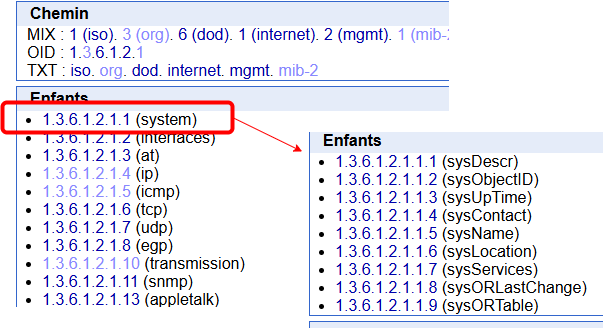
\includegraphics[scale=0.5]{./ressource/exMib}
\end{center}

Exemple d’une MIB (MIB-2, standard SNMP) permettant de décrire le système :
\begin{lstlisting}[style=commande]
1.3.6.1.2.1.1.1 = sysDescr
\end{lstlisting}

Pour intérroger un appareli avec son OID : 
\begin{lstlisting}[style=commande]
$ snmpwalk -v2c -c public 192.168.1.73 1.3.6.1.2.1.1.1

iso.3.6.1.2.1.1.1.0 = STRING: "UAP-nanoHD 6.6.78.15404"
\end{lstlisting}
\subsection*{Fonctionnement}
Les messages échangés incluent :
\begin{itemize}
    \itemE \textbf{GET} : Le gestionnaire interroge un agent pour obtenir une valeur d'un OID particulier
    \item \textbf{GETBULK} : Cette commande permet au gestionnaire de récupérer plusieurs valeurs en une seule requête, ce qui est particulièrement utile pour obtenir des données à partir de table. Elle est plus efficace que de faire plusieurs requêtes GET pour obtenir des informations similaires.
    \itemE \textbf{SET} : Le gestionnaire modifie une valeur sur un agent.
    \itemE \textbf{TRAP} : L’agent envoie une alerte au gestionnaire lorsqu’un événement se produit.
\end{itemize}

\paragraph{Exemple de trame SNMP Get ET GETBULK}
\begin{center}
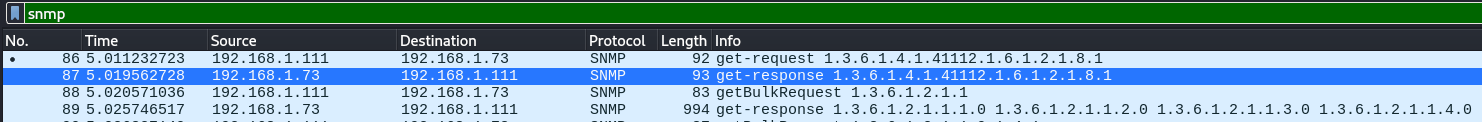
\includegraphics[scale=0.7]{./ressource/exSnmpGet}
\end{center}


\paragraph{Exemple de topologie SNMP}
\begin{center}
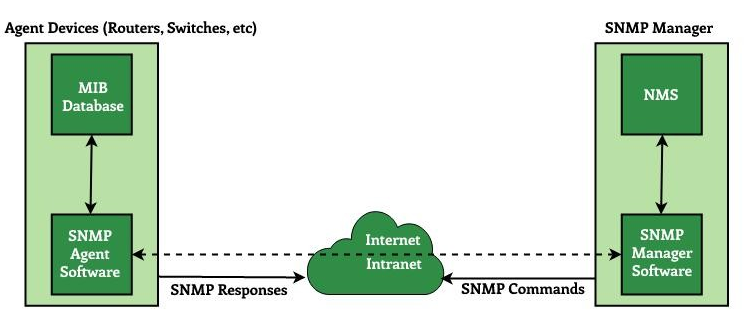
\includegraphics[scale=0.7]{./ressource/SNMP_archi}
\end{center}


\subsection*{Avantages et limites de SNMP}
\textbf{Avantages} :
\begin{itemize}
    \itemE Large compatibilité avec les périphériques réseau.
    \itemE Architecture simple.
\end{itemize}
\textbf{Limites} :
\begin{itemize}
    \itemE Sécurité limitée dans SNMPv1 et SNMPv2.
    \itemE Difficulté d’intégration avec des architectures modernes comme Kubernetes.
\end{itemize}

\section{Zabbix}
Des outils dédiés existent comme \textbf{Zabbix} permettant de gérer les agent SNMP. Il existent plusieurs manière de l'installer dont une via des containers présent sur le dépot : 
\begin{itemize}
\itemE \href{https://github.com/akmalovaa/zabbix-docker}{https://github.com/akmalovaa/zabbix-docker}
\end{itemize}

\begin{center}
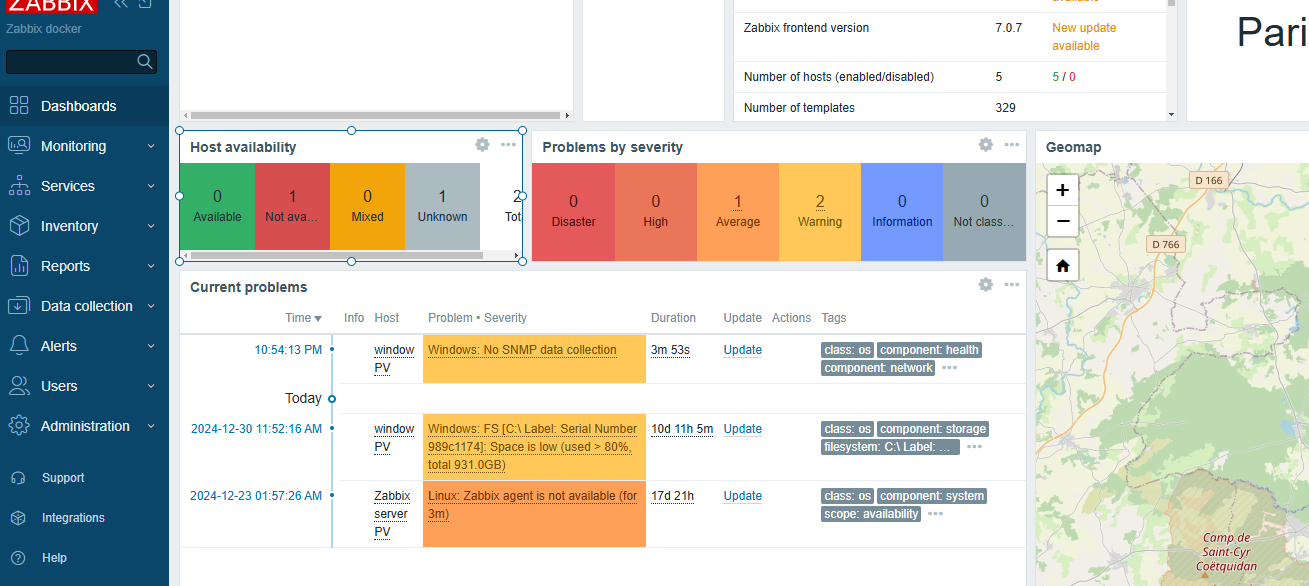
\includegraphics[scale=0.4]{./ressource/zabbix.png}
\end{center}

\begin{center}
 \rule{0.75\linewidth}{1pt}
 \end{center}

\begin{enumerate}
\item Un agent SNMP est présent sur la borne Wifi, d'adresse : 192.168.1.73. Ajouter un host comme présenté ci-dessous. 

\end{enumerate}

\begin{center}
 \rule{0.75\linewidth}{1pt}
 \end{center}

\begin{center}
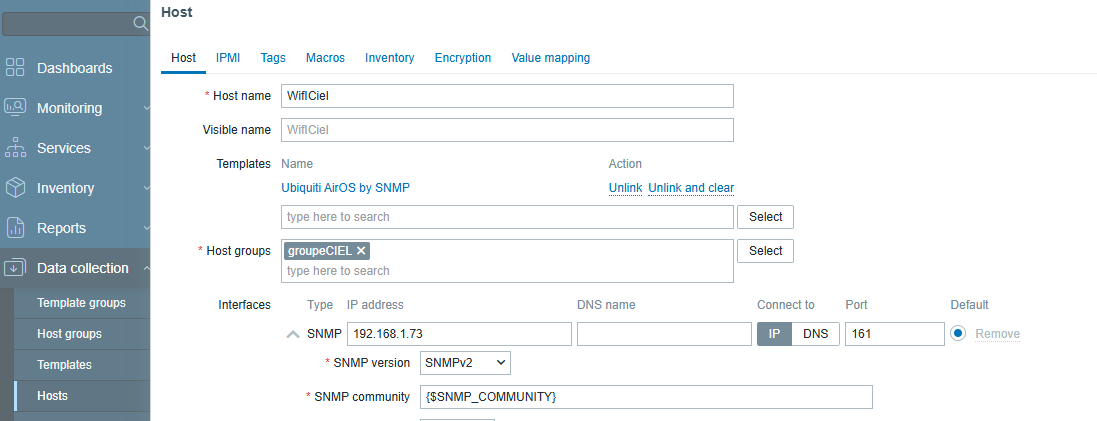
\includegraphics[scale=0.4]{./ressource/wifiSnmp}
\end{center}

\begin{center}
 \rule{0.75\linewidth}{1pt}
 \end{center}

\begin{enumerate}
\item Observer alors avec les outils de monitoring de Zabbix si la borne Wifi fonctionne correctement (j'espère). 
\end{enumerate}

\begin{center}
 \rule{0.75\linewidth}{1pt}
 \end{center}

\begin{center}
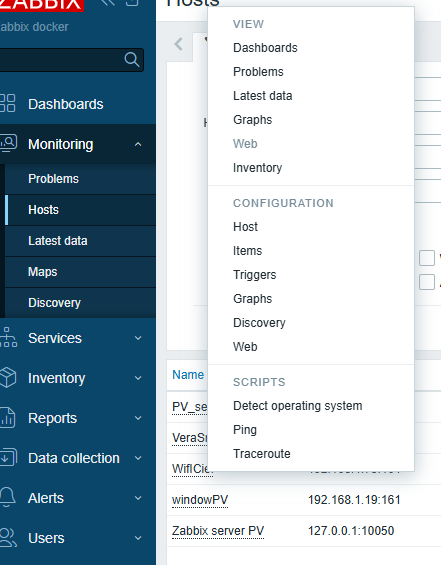
\includegraphics[scale=0.4]{./ressource/zabbixObservation}
\end{center}


\begin{center}
 \rule{0.75\linewidth}{1pt}
 \end{center}

\begin{enumerate}[resume]
\item Avec Wireshark pouvez-vous observez les échanges? Est ce que cela peut convenir? Pourquoi? 
\end{enumerate}

\begin{center}
 \rule{0.75\linewidth}{1pt}
 \end{center}

\ifPROF
\color{red}
NMPv1 et SNMPv2c
Transmission en clair : Les données (y compris les mots de passe, appelés "communautés") sont transmises en clair sur le réseau.
Chiffrement disponible : SNMPv3 introduit des mécanismes de sécurité avancés, notammen

\normalcolor
\fi

\section{SNMP et prometheus}

Il est possible d'utiliser notre \textbf{monitoring stack} pour surveiller des appareils utilisant le SNMB. Pour cela, il faut déjà s'assurer que le SNMP est opérationnel : 

\begin{lstlisting}[style=commande] 
snmpwalk -v2c -c public 192.168.1.73
\end{lstlisting} 

Ensuite,il faut créer un exporter snmp qui va dialoguer avec l'appareil (notre borne Wifi). Pour cela, il faut ajouter un container dans notre \verb?docker-compose.yml?.

\paragraph{Container } \verb?docker-compose.yml?

\begin{lstlisting}[style=commande] 
#Pour SNMP	
  snmp-exporter:
    image: prom/snmp-exporter:latest
    container_name: snmp-exporter
    ports:
      - "9116:9116" # Par defaut, SNMP Exporter ecoute sur le port 9116
    volumes:
      - ./snmp.yml:/etc/snmp_exporter/snmp.yml # Fichier de configuration SNMP
    command:
      - "--config.file=/etc/snmp_exporter/snmp.yml"
    network_mode: "host"
\end{lstlisting} 


\paragraph{Configuration de snmp exporter } \verb?snmp.yml?
Il faut créer un fichier \verb?snmp.yml? et s'assurer qu'il est bien monté dans \verb?volumes? du fichier docker-compose section \verb?snmp-exporter?(c.f au-dessus).  Il doit contenir les lignes suivantes.

\begin{lstlisting}[style=commande] 
auths:
  public_v1:
    version: 1
  public_v2:
    community: public
    security_level: noAuthNoPriv
    auth_protocol: MD5
    priv_protocol: DES
    version: 2

modules:
  snmp-wifi:
    #Parcour l'arbre MIB pour recuperer tous les OID (peut-etre lourd)
    walk:
      - 1.3.6.1.2.1.1       # Description systeme GETBULK
      
    #Juste pour OID precis => Plus lege
    #get:
      #- 1.3.6.1.2.1.1.3   #GET
    
    metrics:
    - name: sysDescr
      oid: 1.3.6.1.2.1.1.1
      type: DisplayString
      help: Nom et descritpion du systeme
    - name: sysUpTime
      oid: 1.3.6.1.2.1.1.3
      type: gauge
      help: Temps depuis la derniere reinit- 1.3.6.1.2.1.1.3  
    timeout: 20s
    retries: 5
\end{lstlisting} 
 
\paragraph{Configuration de prometheus } \verb?prometheus.yml?
Il faut ensuite configurer Prometheus pour ajouter un job 

\begin{lstlisting}[style=commande] 
- job_name: 'snmp-wifi'
    static_configs:
      - targets: ['192.168.1.XX']  # Adresse IP de votre borne WiFi
    metrics_path: /snmp
    params:
      auth: [public_v2]
      module: [snmp-wifi]  # Utilisation du module "default" defini dans snmp.yml
    relabel_configs:
      - source_labels: [__address__]
        target_label: __param_target
      - source_labels: [__param_target]
        target_label: instance
      - target_label: __address__
        replacement: 192.YY.YY.YY:9116  # hostname:port du snmp reporter (IP+Port)
\end{lstlisting} 


\paragraph{Résultat dans Prometheus}
 
Normalement, vous devez voir dans prometheus le job \textbf{snmp-wifi}

\begin{center}
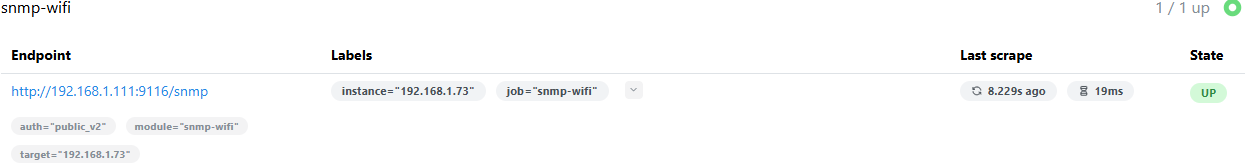
\includegraphics[scale=0.5]{./ressource/snmpWifi}
\end{center}

Et en regardant les détails  (l'adresse mon serveur est 192.168.1.111 et le snmp-exporter écoute sur le port 9116).
\begin{center}
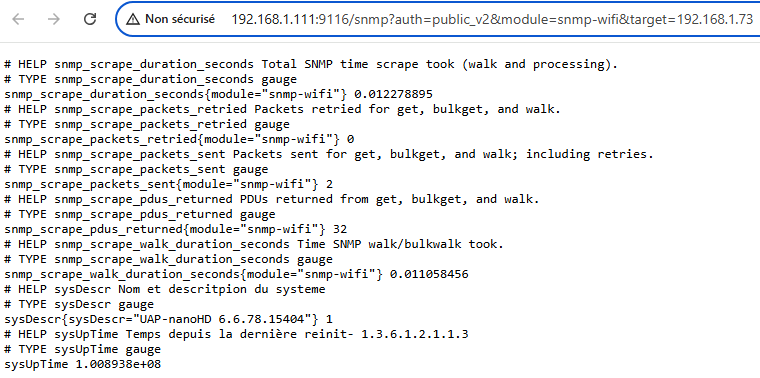
\includegraphics[scale=0.7]{./ressource/detailsSnmpWifi}
\end{center}

 
\paragraph{Détails supplémentaires pour le fichier snmp.yml} \  

\href{https://github.com/prometheus/snmp_exporter/blob/main/snmp.yml}{https://github.com/prometheus/snmp\_exporter/blob/main/snmp.yml}


\section{A vous}
L'OID 1.3.6.1.4.1.41112.1.6.1.2.1.8.1 correspond au nombre de personnes connectées à la borne WIFI \textbf{UAP-nanoHD}

\begin{enumerate}
\item Avec une commande appropriée, vérifier cette information. 
\item Ajouter dans Prometheus cette métrique
\item Dans Grafana, Visualiser cette métrique
\end{enumerate}

\ifPROF
\color{red}
\begin{lstlisting}[style=commande] 
#snmpwalk -v2c -c public 192.168.1.73 1.3.6.1.4.1.41112.1.6.1.2.1.8.1
snmpwalk -v2c -c public 192.168.1.31 1.3.6.1.4.1.41112.1.6.1.2.1.8.2
\end{lstlisting}
\normalcolor
\fi

\end{document}
